Bending machine is set to operate automatically by controlling the foot pedal with \hyperref[acro:PLC]{PLC}.
To automate the bending process, several devices and components are installed on the bending machine.
Bending machine is operated freely up to a certain point \textit{i.e.} without any pressure and only starts
applying pressure when it is in contact with the sheet metal part.
Figure \ref{fig:bending_machine} shows these components.


\subsubsection{Marker}
\label{subsubsec:marker}
Detection marker mounted on the bending machine. This pose is used as reference frame for all three bending stations.
Since the bending machine is fixed, this marker is also used for auto calibration of the robotic camera.


\begin{figure}[h]
    \centering
    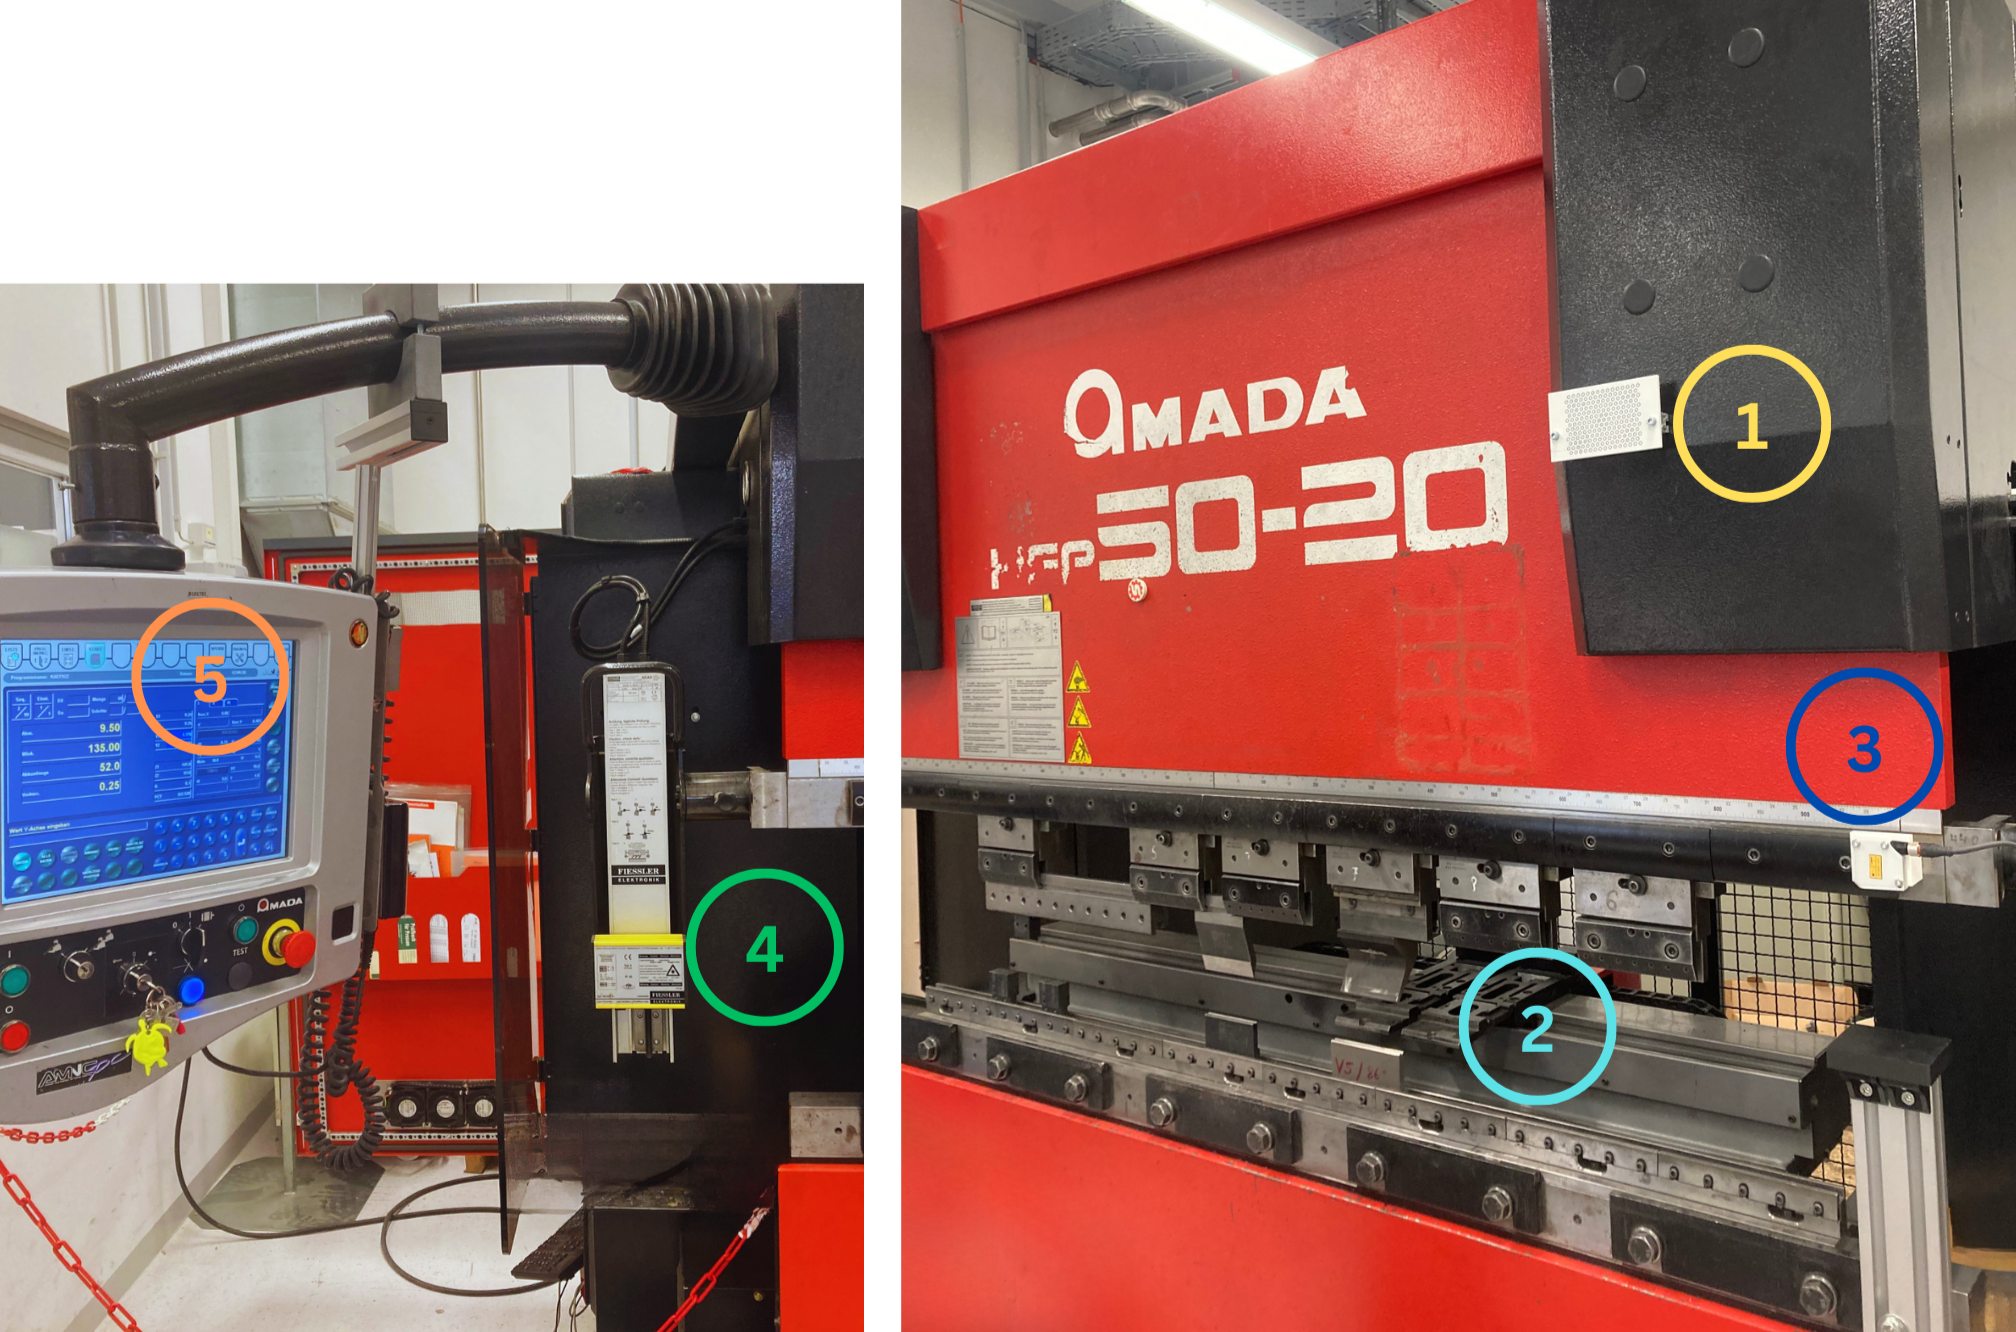
\includegraphics[width=1\textwidth]{figures/bending-machine.png}
    \caption{\hyperref[acro:AMADA]{AMADA} Bending Machine. 1) Marker  2) Bending machine open height measurement sensor 3) Bending station 4) Terminal fixture 5) Laser monitoring}
    \label{fig:bending_machine}
\end{figure}

\subsubsection{Bending machine open height measurement sensor}
\label{subsubsec:laser-sensor}

It is important to know exactly the current open height of the bending machine.
This value tells the \hyperref[acro:KR]{KR} to open the pneumatic parallel gripper as sheet starts bending at a bending station to avoid any deformation in the sheet.
Once the bending is complete, the \hyperref[acro:KR]{KR} can move out safely without any collision if a set-point on the open height is reached.

For this, a laser sensor is mounted on the bending machine which measures the open height of the bending machine.
The sensor values are sent to the \hyperref[acro:PLC]{PLC}. \hyperref[acro:KR]{KR} makes decision to do bending operation based on this laser sensor value.


\subsubsection{Bending station}
\label{subsubsec:bending-station}
There are three bending stations in the bending machine. Each bending station has a different set of punch and die.
Bending station 1 is used to achieve a bending of 90\textdegree. Bending station 2 bends the sheet metal part at an angle of 135\textdegree.
And finally, bending station is used to press down the sheet and make it flat.

\begin{figure}[h]
    \centering
    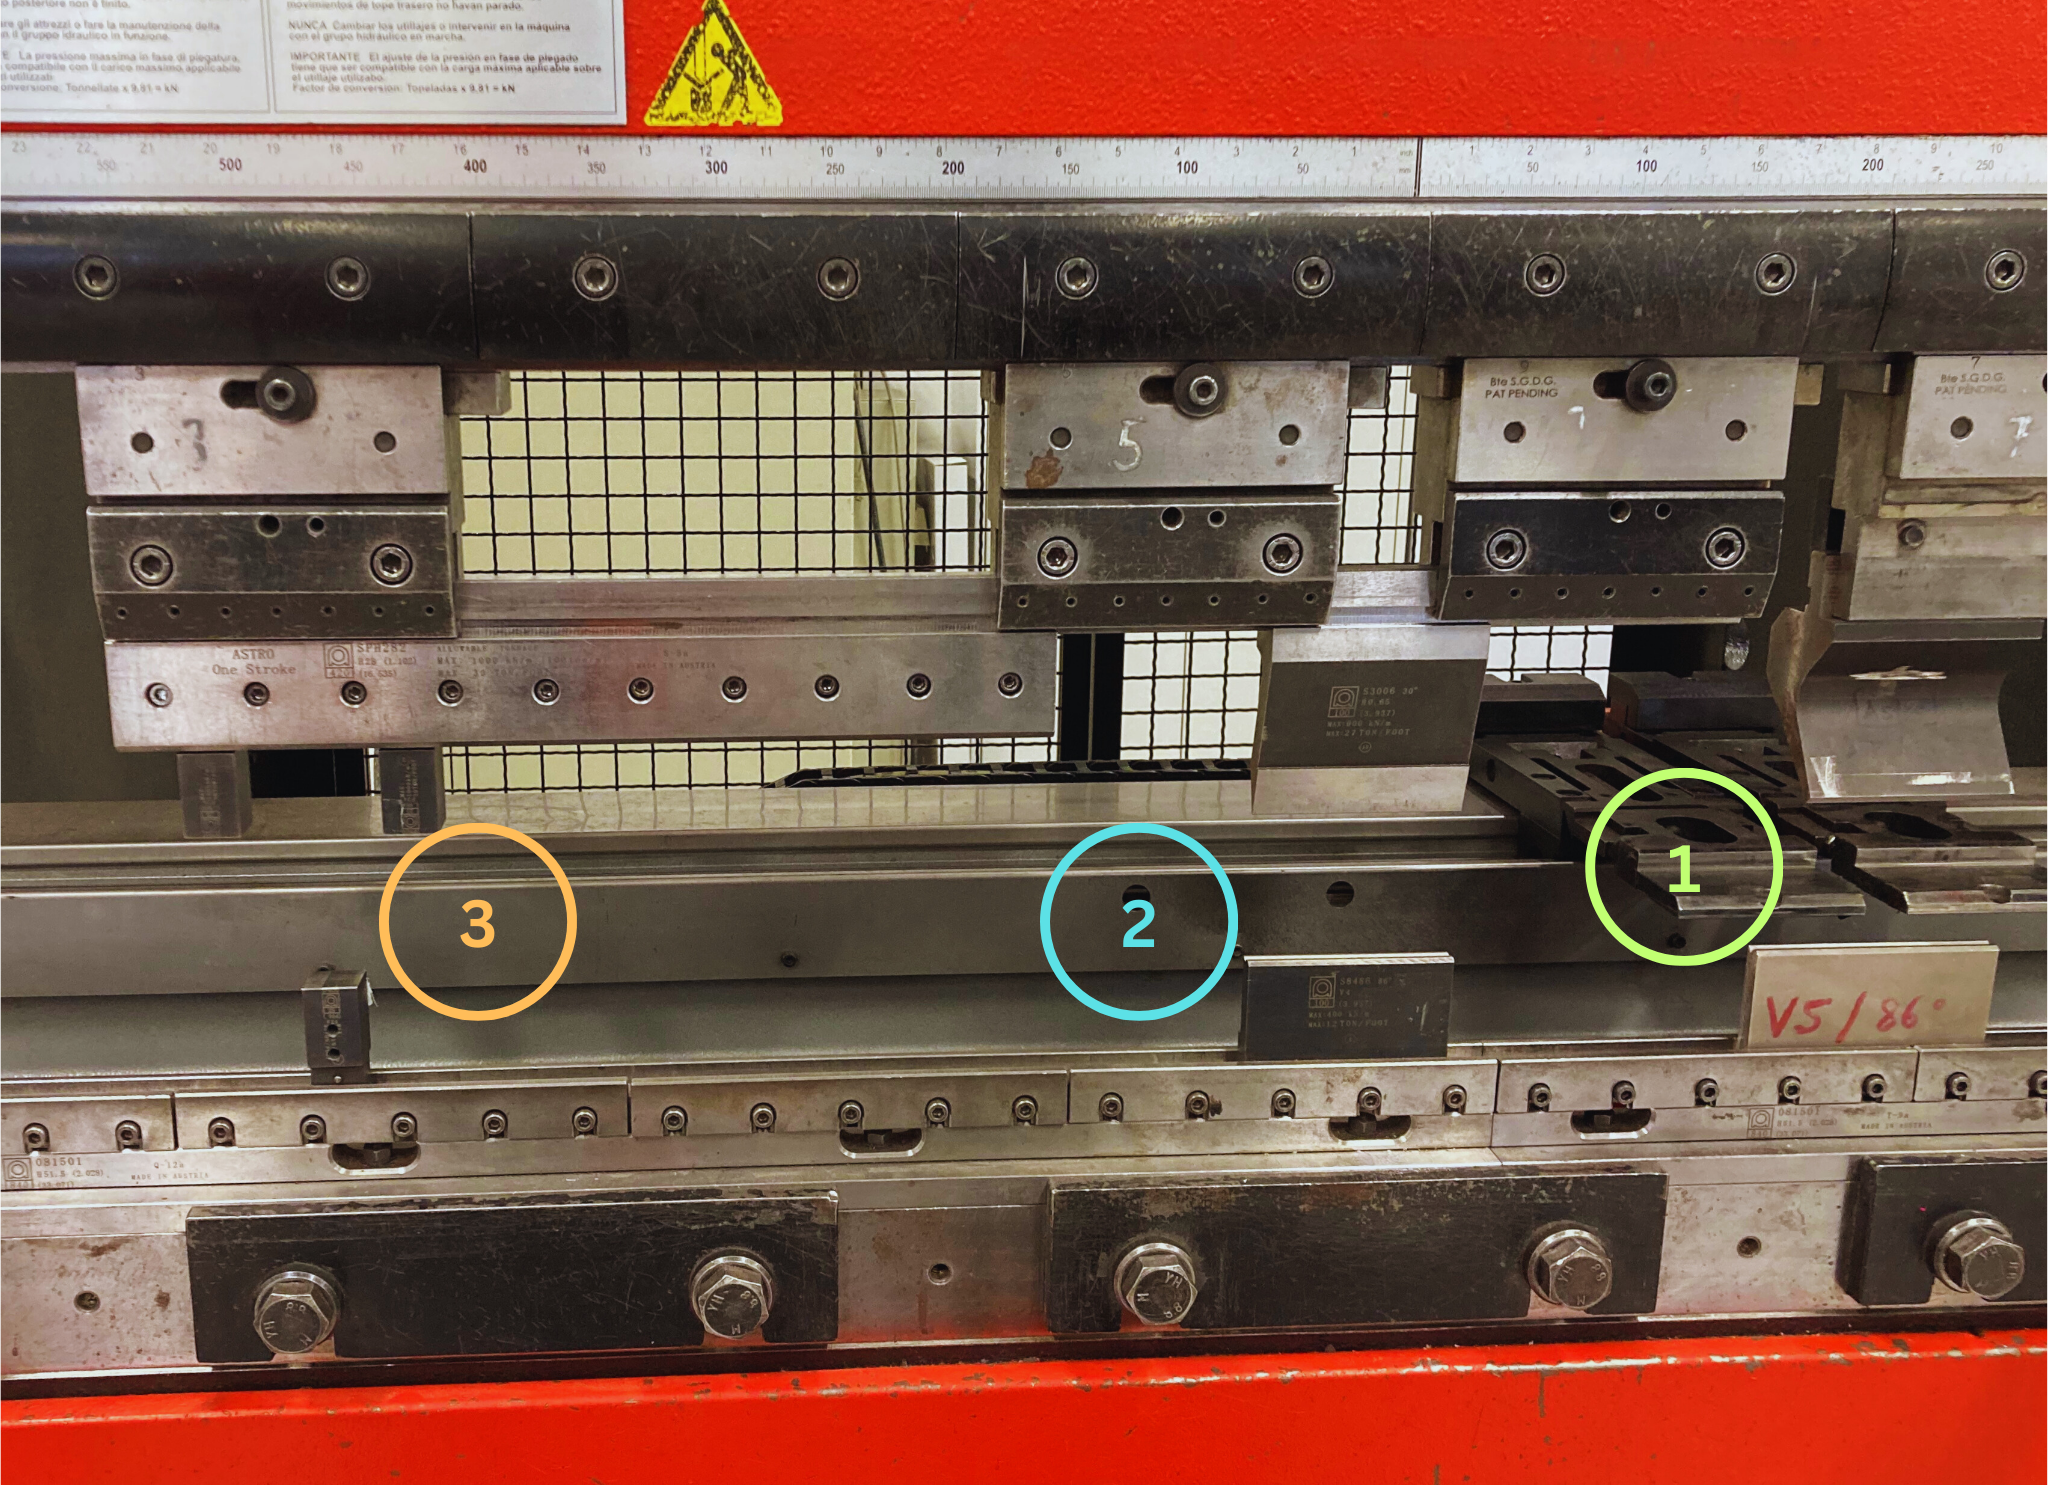
\includegraphics[width=0.7\textwidth]{figures/bending-station.png}
    \caption{Three bending stations for the bending operation}
    \label{fig:bending-station}
\end{figure}

These three stations are enough for the sheet bending operation. \hyperref[acro:KR]{KR1410} will take the sheet metal part to one of these bending station
to perform a bending of a particular angle. A sheet metal part could require the use of one or more of these bending stations.

\subsubsection{Terminal Fixture}
The bending machine comes with a terminal which is used to operate the bending machine. However, this terminal is free to rotate and move.
It is required to fix the movement of terminal, so that terminal operating robot could operate reliably. The fixtures made from aluminum profiles fixes the bending machine
terminal.
